% ==========================================
% BAB IV PERANCANGAN (DESAIN KONSEP SOLUSI)
% ==========================================
\cleardoublepage
\chapter{PERANCANGAN SISTEM \textit{BUSINESS INTELLIGENCE CHATBOT}}
\label{chap:perancangan}

Berdasarkan analisis komprehensif terhadap permasalahan yang dihadapi dan kebutuhan pengguna yang telah diuraikan pada bab-bab sebelumnya, penelitian ini mengajukan solusi terintegrasi berupa \textit{Business Intelligence Chatbot System} berbasis teknologi pembelajaran mendalam (\textit{deep learning}) yang menggabungkan tiga komponen utama, yaitu mekanisme pencocokan pola (\textit{pattern-based intent classification}) untuk pemahaman maksud pengguna, mesin kueri berbasis aturan (\textit{rule-based query engine}) untuk pengambilan data terstruktur, serta model peramalan deret waktu (\textit{time series forecasting}) untuk analisis prediktif. Solusi yang diajukan dirancang dengan visi untuk menghilangkan hambatan aksesibilitas data analitik bagi pengguna nonteknis melalui antarmuka percakapan yang intuitif dan responsif dalam bahasa alami, sekaligus meningkatkan kecepatan pengambilan keputusan melalui otomatisasi proses analisis dan pelaporan. Sistem ini mengintegrasikan kemampuan deskriptif, diagnostik, dan prediktif dalam satu \textit{platform} terpadu yang memanfaatkan infrastruktur \textit{Enterprise Data Warehouse} yang telah ada sehingga meminimalkan disrupsi terhadap operasional bisnis yang sedang berjalan dan mengurangi kebutuhan perubahan drastis pada lanskap teknologi eksisting.

Transformasi dari kondisi \textit{status quo} menuju solusi yang diusulkan melibatkan perubahan yang bersifat fundamental pada tiga aspek utama, yaitu arsitektur sistem yang bergeser dari pelaporan manual dan \textit{dashboard} statis menuju sistem otomatis berbasis percakapan dengan kemampuan pemrosesan mendekati \textit{real-time}, kemampuan analitik yang berkembang dari analisis retrospektif menjadi analisis prediktif yang bersifat proaktif, serta pengalaman pengguna yang beralih dari ketergantungan pada pengguna teknis yang memahami SQL menjadi kemudahan akses bagi pengguna bisnis umum melalui interaksi berbasis bahasa alami. Dengan demikian, sistem diharapkan mampu menjembatani kesenjangan antara kebutuhan pengambilan keputusan yang cepat dan kompleksitas teknis yang selama ini menjadi penghalang utama dalam pemanfaatan penuh kapabilitas data dan analitik di lingkungan organisasi.

Sistem analitik yang ada saat ini (\textit{as-is}) masih mengikuti pola operasional tradisional yang berfokus pada pelaporan manual dan eksplorasi data yang terbatas. Proses dimulai dari identifikasi kebutuhan analitik oleh pengguna bisnis, dilanjutkan dengan penerjemahan kebutuhan tersebut menjadi kueri basis data oleh analis atau tim teknis, eksekusi kueri terhadap \textit{Enterprise Data Warehouse}, pemrosesan dan transformasi data untuk memenuhi standar kualitas serta format analisis, kemudian diakhiri dengan penyajian hasil dalam bentuk laporan atau visualisasi \textit{dashboard}. Keterbatasan utama dari pola \textit{as-is} ini mencakup waktu respons yang lama akibat proses multi-tahap dengan \textit{multiple touchpoint} antardepartemen sebelum \textit{insight} dapat dihasilkan, tingkat aksesibilitas yang rendah karena hanya pengguna dengan keahlian teknis yang mampu melakukan analisis secara mandiri, ketiadaan kemampuan prediktif karena sistem berfokus pada analisis historis tanpa dukungan \textit{forecasting} untuk pengambilan keputusan proaktif, serta efisiensi operasional yang rendah karena tim teknis harus mengalokasikan waktu signifikan untuk mengonversi permintaan analitik menjadi \textit{query} teknis alih-alih berfokus pada aktivitas bernilai tambah yang lebih strategis.

\section{Alur Proses Bisnis Sistem Analitik Saat Ini (\textit{As-Is})}
\label{sec:asis}

Proses bisnis sistem analitik saat ini direpresentasikan dalam notasi BPMN (\textit{Business Process Model and Notation}) yang menggambarkan interaksi antar aktor, keputusan-keputusan kritis, dan aliran data dalam organisasi. Proses dimulai dengan identifikasi kebutuhan analisis baru oleh pengguna bisnis, dilanjutkan dengan klarifikasi kebutuhan dan pengembangan \textit{query} oleh tim teknis, eksekusi \textit{query} pada \textit{data warehouse}, pemrosesan data hasil \textit{query}, pembangunan \textit{dashboard} atau laporan, \textit{review} dan validasi internal, iterasi perbaikan apabila diperlukan, serta diakhiri dengan publikasi hasil analisis kepada pengguna akhir. Di dalam alur tersebut terdapat beberapa titik keputusan (\textit{decision point}) yang bersifat kritis, antara lain: apakah permintaan dapat dipenuhi dengan \textit{dashboard existing} atau memerlukan \textit{custom query}, apakah data hasil \textit{query} sudah sesuai dengan ekspektasi pengguna atau memerlukan transformasi tambahan, serta apakah hasil analisis sudah valid untuk dipublikasikan atau masih memerlukan revisi. Proses \textit{as-is} ini bersifat iteratif dengan siklus umpan balik yang panjang dan kurang efisien dalam memenuhi kebutuhan analitik yang dinamis dan beragam dari pengguna bisnis. Diagram BPMN yang menggambarkan proses \textit{as-is} disajikan pada Gambar~\ref{fig:bpmnasis}.

\begin{figure}[htbp] 
  \centering
  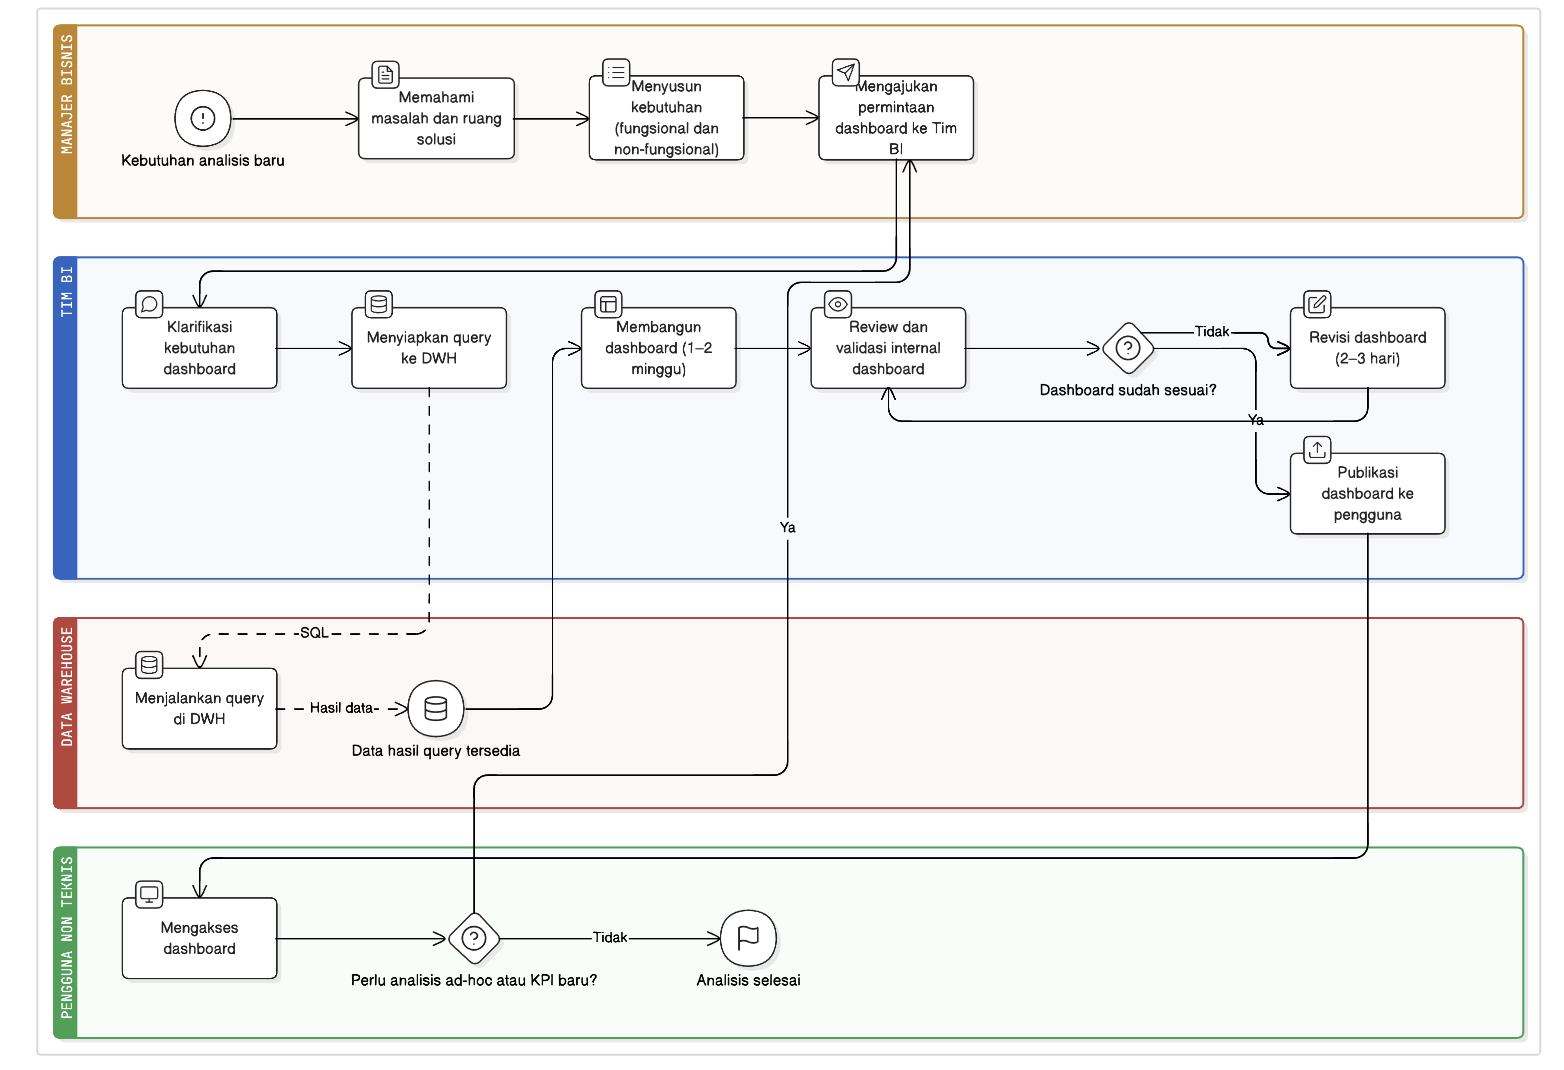
\includegraphics[width=1\textwidth,
                   height=1\textheight,
                   keepaspectratio]{images/bpmnasis}
  \caption{BPMN Sistem \textit{As-Is}}
  \label{fig:bpmnasis}
\end{figure}

Visualisasi proses \textit{as-is} menunjukkan kompleksitas dan iterasi yang terlibat dalam setiap siklus permintaan analitik. Pengguna bisnis harus menunggu beberapa tahap pemrosesan, \textit{review}, dan validasi sebelum hasil analisis dapat diakses. Aliran data bersifat linear dengan berbagai \textit{handoff} antar departemen sehingga menciptakan \textit{bottleneck} dan jeda yang signifikan. Pengalaman pengguna berpusat pada antarmuka \textit{dashboard} statis, tanpa kemampuan untuk melakukan eksplorasi data secara interaktif maupun berinteraksi melalui dialog percakapan yang natural.

\section{Alur Proses Bisnis Sistem Analitik dengan Chatbot BI (\textit{To-Be})}
\label{sec:tobe}

Proses bisnis sistem analitik yang diusulkan (\textit{to-be}) merepresentasikan tingkat otomatisasi dan optimasi yang signifikan dibandingkan proses \textit{as-is}. Proses dimulai ketika pengguna mengajukan pertanyaan dalam bahasa alami kepada sistem \textit{chatbot}, yang kemudian dilanjutkan dengan proses \textit{login} ke sistem \textit{BI chatbot} untuk keperluan autentikasi dan otorisasi pengguna. Setelah autentikasi berhasil, sistem membangun halaman dialog \textit{chatbot} sebagai antarmuka utama interaksi antara pengguna dan sistem yang bersifat \textit{AI-powered}. Tahap pemrosesan dimulai dengan klasifikasi maksud berbasis pola untuk mengidentifikasi jenis pertanyaan yang diajukan, apakah bersifat deskriptif, diagnostik, atau prediktif. Berdasarkan jenis \textit{intent} tersebut, sistem melakukan perutean (\textit{routing}) ke modul yang sesuai, yaitu untuk analisis deskriptif dan diagnostik, sistem menggunakan \textit{rule-based query engine} untuk menghasilkan dan mengeksekusi kueri terstruktur terhadap \textit{data warehouse}; sedangkan untuk analisis prediktif, sistem mengakses model \textit{forecasting} yang telah dilatih untuk menghasilkan prediksi sesuai dengan rentang waktu (\textit{time horizon}) dan parameter yang relevan. Setelah hasil analisis diperoleh, sistem melakukan perhitungan KPI dan agregasi data, kemudian menerapkan \textit{natural language generation} berbasis templat (\textit{template-based NLG}) untuk mengonversi keluaran numerik menjadi narasi dalam bahasa alami yang koheren dan mudah dipahami. Respons yang telah diformat dalam Bahasa Indonesia kemudian ditampilkan kembali kepada pengguna melalui antarmuka \textit{chatbot}, dan pada tahap akhir pengguna dapat mengakses \textit{dashboard} untuk melakukan \textit{ad-hoc analysis} atau pelacakan KPI tambahan apabila diperlukan, atau proses diakhiri ketika analisis dinyatakan selesai.

Keunggulan proses \textit{to-be} dibandingkan proses \textit{as-is} terletak pada beberapa aspek utama: \textbf{kecepatan eksekusi} yang jauh lebih tinggi (hitungan menit dibandingkan hari) berkat eksekusi kueri \textit{real-time}, \textbf{aksesibilitas yang lebih luas} karena tidak lagi memerlukan keahlian teknis SQL untuk mengakses \textit{insight}, \textbf{otomatisasi proses} yang mengurangi beban kerja manual tim teknis melalui pemanfaatan \textit{rule-based query} dan penanganan \textit{intent} otomatis, \textbf{kemampuan analitik yang diperluas} melalui integrasi komponen prediktif berbasis \textit{machine learning}, serta \textbf{pengalaman pengguna} yang lebih baik melalui antarmuka percakapan yang natural dan responsif. Secara keseluruhan, rancangan \textit{to-be} ini memungkinkan siklus permintaan hingga penyajian hasil analitik standar diselesaikan dalam waktu kurang dari satu menit untuk mayoritas kasus sehingga lebih selaras dengan kebutuhan pengambilan keputusan yang cepat dan berbasis data. Diagram BPMN yang menggambarkan proses \textit{to-be} disajikan pada Gambar~\ref{fig:bpmntobe}.

\begin{figure}[htbp] 
  \centering
  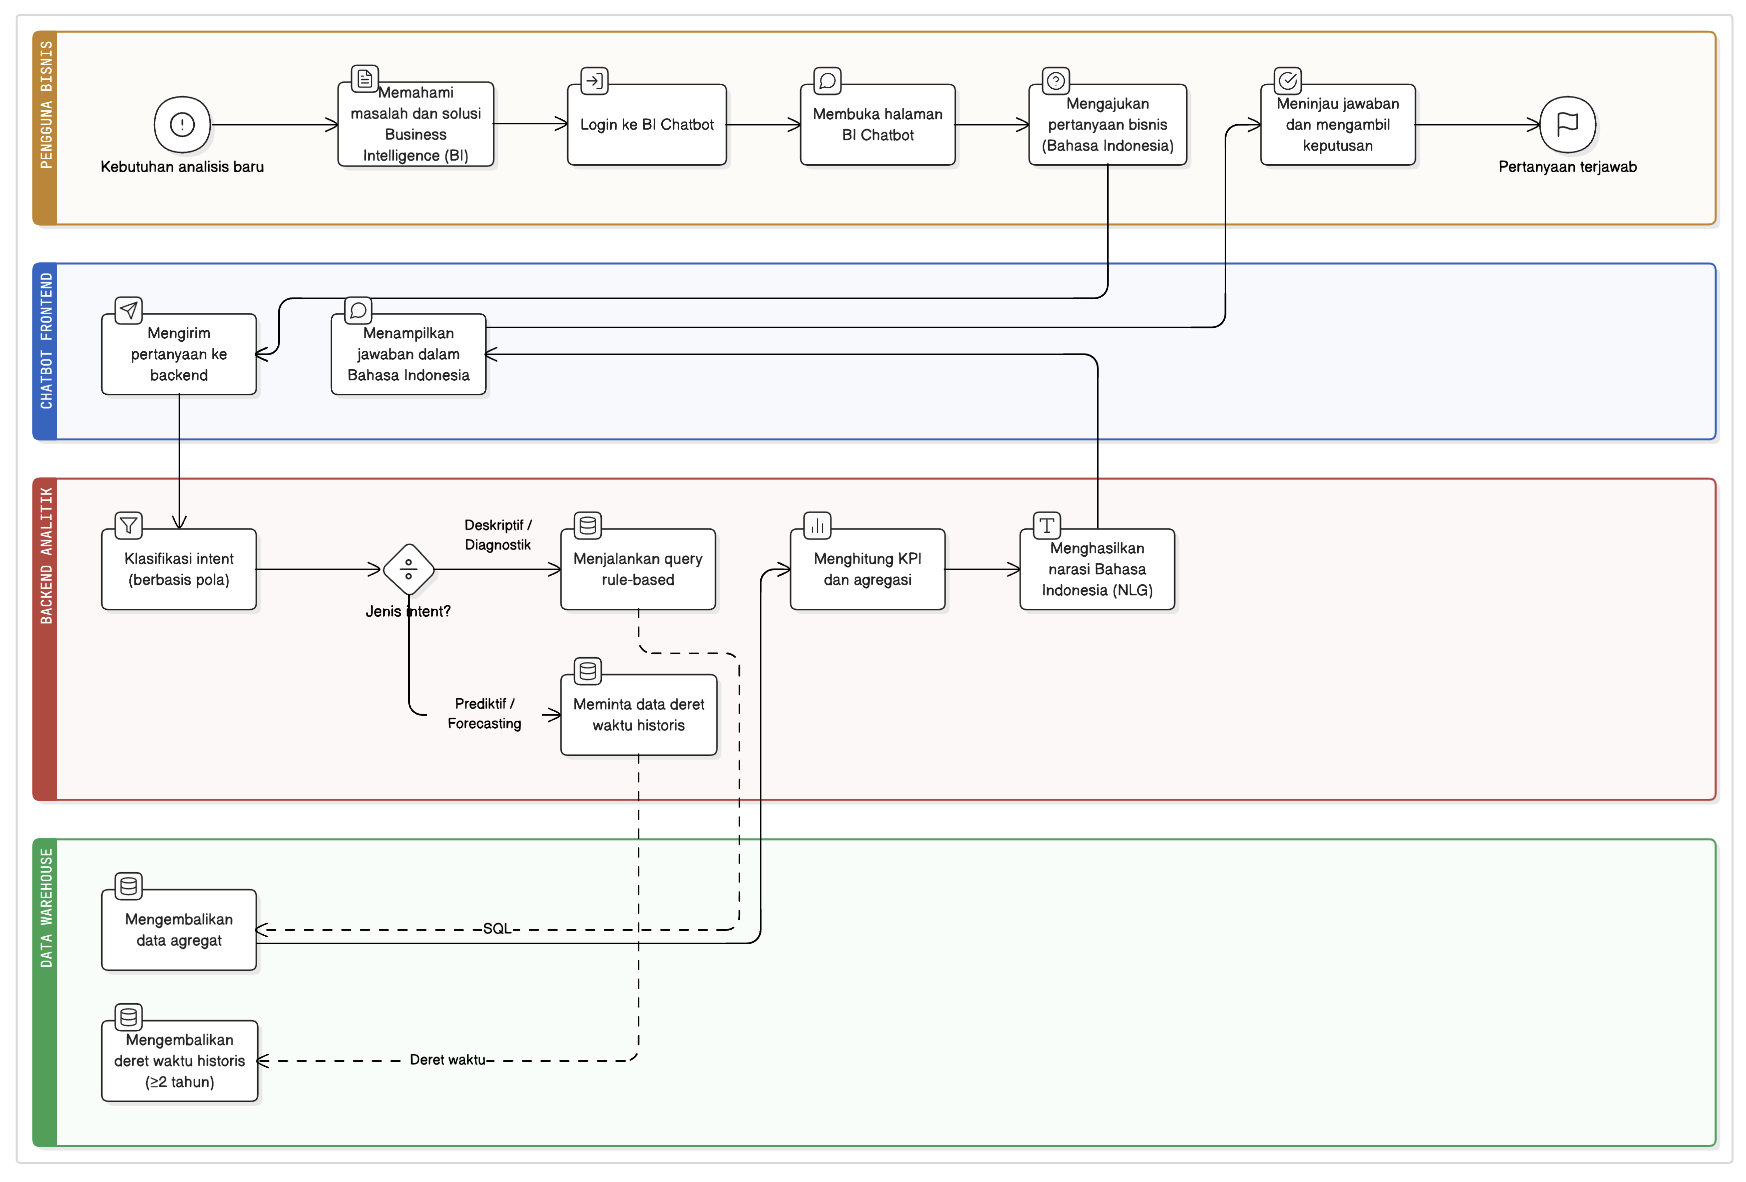
\includegraphics[width=1\textwidth,
                   height=1\textheight,
                   keepaspectratio]{images/bpmntobe}
  \caption{BPMN Sistem \textit{To-Be}}
  \label{fig:bpmntobe}
\end{figure}

Visualisasi proses \textit{to-be} menunjukkan peningkatan yang signifikan dalam efisiensi dan responsivitas sistem. Pengguna dapat secara langsung mengajukan pertanyaan melalui antarmuka \textit{chatbot} tanpa perlu menunggu atau melibatkan tim teknis. Aliran data bersifat paralel dengan otomatisasi penuh pada tahap pemrosesan sehingga memungkinkan hasil analisis diterima dalam waktu yang sangat singkat. Pengalaman pengguna berpusat pada dialog percakapan yang interaktif, dengan kemampuan untuk melakukan eksplorasi data secara \textit{real-time} serta mengajukan kueri lanjutan (\textit{follow-up queries}) secara mulus.

\section{Perbandingan Sistem Saat Ini (\textit{As-Is}) dan Sistem Baru (\textit{To-Be})}
\label{sec:perbandingan-asis-tobe}

Berdasarkan analisis proses bisnis yang telah diuraikan pada bagian sebelumnya, terdapat perbedaan fundamental antara sistem analitik saat ini (\textit{as-is}) dan sistem yang diusulkan (\textit{to-be}). Sistem \textit{as-is} mengandalkan pelaporan manual dengan keterlibatan tim teknis pada setiap tahap, sedangkan sistem \textit{to-be} mengotomatisasi sebagian besar proses melalui antarmuka percakapan berbasis \textit{chatbot}. Perbandingan kedua sistem berdasarkan aspek-aspek kritis disajikan pada Tabel~\ref{tab:perbandingan-asis-tobe}.

\begin{longtable}{|p{2.5cm}|p{5.5cm}|p{5.5cm}|}
\caption{Perbandingan Sistem \textit{As-Is} dan \textit{To-Be}} \label{tab:perbandingan-asis-tobe} \\
\hline
\textbf{Aspek} & \textbf{Sistem \textit{As-Is}} & \textbf{Sistem \textit{To-Be}} \\
\hline
\endfirsthead
\multicolumn{3}{c}{\tablename\ \thetable\ -- \textit{Lanjutan dari halaman sebelumnya}} \\
\hline
\textbf{Aspek} & \textbf{Sistem \textit{As-Is}} & \textbf{Sistem \textit{To-Be}} \\
\hline
\endhead
\hline \multicolumn{3}{r}{\textit{Bersambung ke halaman berikutnya}} \\
\endfoot
\hline
\endlastfoot

Waktu Respons & 2--5 hari untuk kueri kompleks & $<$2 menit untuk 95\% kueri \\
\hline

Antarmuka Pengguna & \textit{Dashboard} statis, laporan manual & Antarmuka percakapan (\textit{chatbot}) dalam Bahasa Indonesia \\
\hline

Ketergantungan Teknis & Memerlukan tim TI/analis data untuk setiap permintaan & Pengguna nonteknis dapat mengakses \textit{insight} secara mandiri \\
\hline

Aksesibilitas & Terbatas pada pengguna dengan keahlian SQL & Seluruh pengguna internal dapat mengakses melalui bahasa alami \\
\hline

Kemampuan Analitik & Deskriptif dan diagnostik (historis) & Deskriptif, diagnostik, dan prediktif (\textit{forecasting}) \\
\hline

Proses Pengambilan Data & Ekstraksi manual dari berbagai sistem, transformasi via \textit{spreadsheet} & Otomatis melalui \textit{rule-based query engine} \\
\hline

Kemampuan Prediktif & Tidak tersedia atau dilakukan manual secara periodik & Terintegrasi dengan model \textit{time series forecasting} (LSTM/GRU/Prophet/ARIMA) \\
\hline

Format Respons & Tabel, grafik, laporan tertulis & Narasi bahasa alami (\textit{template-based NLG}) dengan visualisasi pendukung \\
\hline

Siklus \textit{Feedback} & Iteratif dan panjang dengan banyak \textit{handoff} & \textit{Real-time} dengan kemampuan kueri lanjutan \\
\hline

Skalabilitas & Terbatas oleh kapasitas tim teknis & Skala horizontal melalui arsitektur layanan mikro \\
\hline

Ketersediaan & Jam kerja (bergantung pada tim teknis) & Diakses setiap saat (\textit{self-service}) \\
\hline

\end{longtable}


\section{Rancangan Solusi Keseluruhan}
\label{sec:rancangan-solusi}

Rancangan solusi keseluruhan mengintegrasikan lima lapisan (\textit{layer}) arsitektur yang saling terhubung, yakni lapisan presentasi (\textit{presentation layer}), lapisan aplikasi (\textit{application layer}), lapisan logika bisnis (\textit{business logic layer}), lapisan data (\textit{data layer}), dan lapisan infrastruktur (\textit{infrastructure layer}). Integrasi kelima lapisan tersebut memastikan bahwa sistem memiliki tingkat fleksibilitas, skalabilitas, dan kemudahan pemeliharaan (\textit{maintainability}) yang tinggi untuk mendukung pertumbuhan bisnis serta evolusi kebutuhan analitik di masa depan.

\subsection{Komponen-Komponen Utama Arsitektur}
\label{subsec:komponen-arsitektur}

Lapisan presentasi mencakup antarmuka pengguna yang dibangun dengan teknologi \textit{web} modern, dengan fokus pada antarmuka \textit{chatbot} berbasis \textit{web} yang mendukung interaksi waktu nyata (\textit{real-time}) dengan \textit{backend} sistem. Antarmuka ini diimplementasikan menggunakan kerangka kerja \textit{frontend} modern dengan pemanfaatan komunikasi asinkronus yang memungkinkan percakapan dua arah tanpa penundaan yang signifikan. Lapisan ini juga mencakup komponen untuk menampilkan visualisasi data, metrik interaktif, dan laporan yang terintegrasi dengan hasil analisis yang dihasilkan oleh \textit{backend}.

Lapisan aplikasi mengenkapsulasi logika inti sistem yang terdiri atas beberapa modul utama. Modul \textit{Natural Language Understanding} (NLU) bertanggung jawab untuk melakukan penguraian (\textit{parsing}) dan pemahaman terhadap masukan pengguna dalam bahasa alami. Modul manajemen dialog mengelola status percakapan dan menjaga koherensi dalam dialog multigiliran (\textit{multi-turn}). Modul pembangkitan respons menghasilkan tanggapan yang sesuai berdasarkan hasil analisis yang diterima dari lapisan logika bisnis. Di sisi lain, lapisan logika bisnis mencakup implementasi aturan bisnis yang telah didefinisikan, mesin klasifikasi maksud, mesin kueri berbasis aturan, model \textit{machine learning} untuk peramalan, serta repositori templat untuk NLG. Lapisan ini merupakan jantung sistem yang mengonversi maksud pengguna menjadi aksi teknis yang konkret dan menghasilkan wawasan berbasis data.

Lapisan data mencakup koneksi dan interaksi dengan \textit{Enterprise Data Warehouse} yang menyimpan data transaksional dan data utama, serta lapisan singgahan (\textit{cache}) untuk menyimpan hasil kueri yang sering diakses guna meningkatkan performa. Lapisan ini juga mencakup repositori untuk menyimpan model \textit{machine learning} yang telah dilatih, metadata mengenai sumber data, dan log audit untuk melacak seluruh interaksi pengguna dengan sistem. Lapisan infrastruktur mencakup komponen teknis yang mendukung operasional sistem secara keseluruhan, antara lain \textit{web server} untuk aplikasi \textit{chatbot}, infrastruktur API untuk penanganan permintaan, layanan pemantauan (\textit{monitoring}) dan pencatatan (\textit{logging}), serta komponen keamanan untuk autentikasi dan otorisasi pengguna.

\subsection{Arsitektur Sistem dan Aliran Data}
\label{subsec:arsitektur-aliran-data}

Arsitektur sistem secara keseluruhan dirancang dengan pendekatan modular berbasis layanan, dengan setiap komponen fungsional (seperti layanan \textit{chatbot}, layanan kueri, layanan peramalan, dan layanan NLG) diimplementasikan secara terpisah. Komunikasi antarkomponen dilakukan melalui API REST untuk memastikan keterikatan yang longgar (\textit{loose coupling}) dan tingkat ketahanan (\textit{resilience}) yang memadai terhadap gangguan.

Diagram arsitektur sistem yang lebih rinci disajikan pada Gambar~\ref{fig:arsitektur}, yang memperlihatkan integrasi kelima lapisan dan aliran data antarkomponen di dalam sistem. Arsitektur ini dirancang untuk mendukung:

\begin{enumerate}
    \item \textbf{Skalabilitas horizontal}, dengan setiap layanan dapat diduplikasi sesuai dengan kebutuhan kapasitas.
    \item \textbf{Ketahanan (\textit{Resilience})} sehingga kegagalan pada satu layanan tidak secara langsung menyebabkan kegagalan sistem secara keseluruhan.
    \item \textbf{Kemudahan Pemeliharaan} karena setiap modul dapat dikembangkan, diuji, dan di-\textit{deploy} secara independen.
    \item \textbf{Interoperabilitas}, melalui kemampuan setiap layanan untuk berinteraksi menggunakan standar API.
    \item \textbf{Keamanan}, dengan penerapan autentikasi berlapis dan enkripsi data.
\end{enumerate}

\begin{figure}[htbp] 
  \centering
  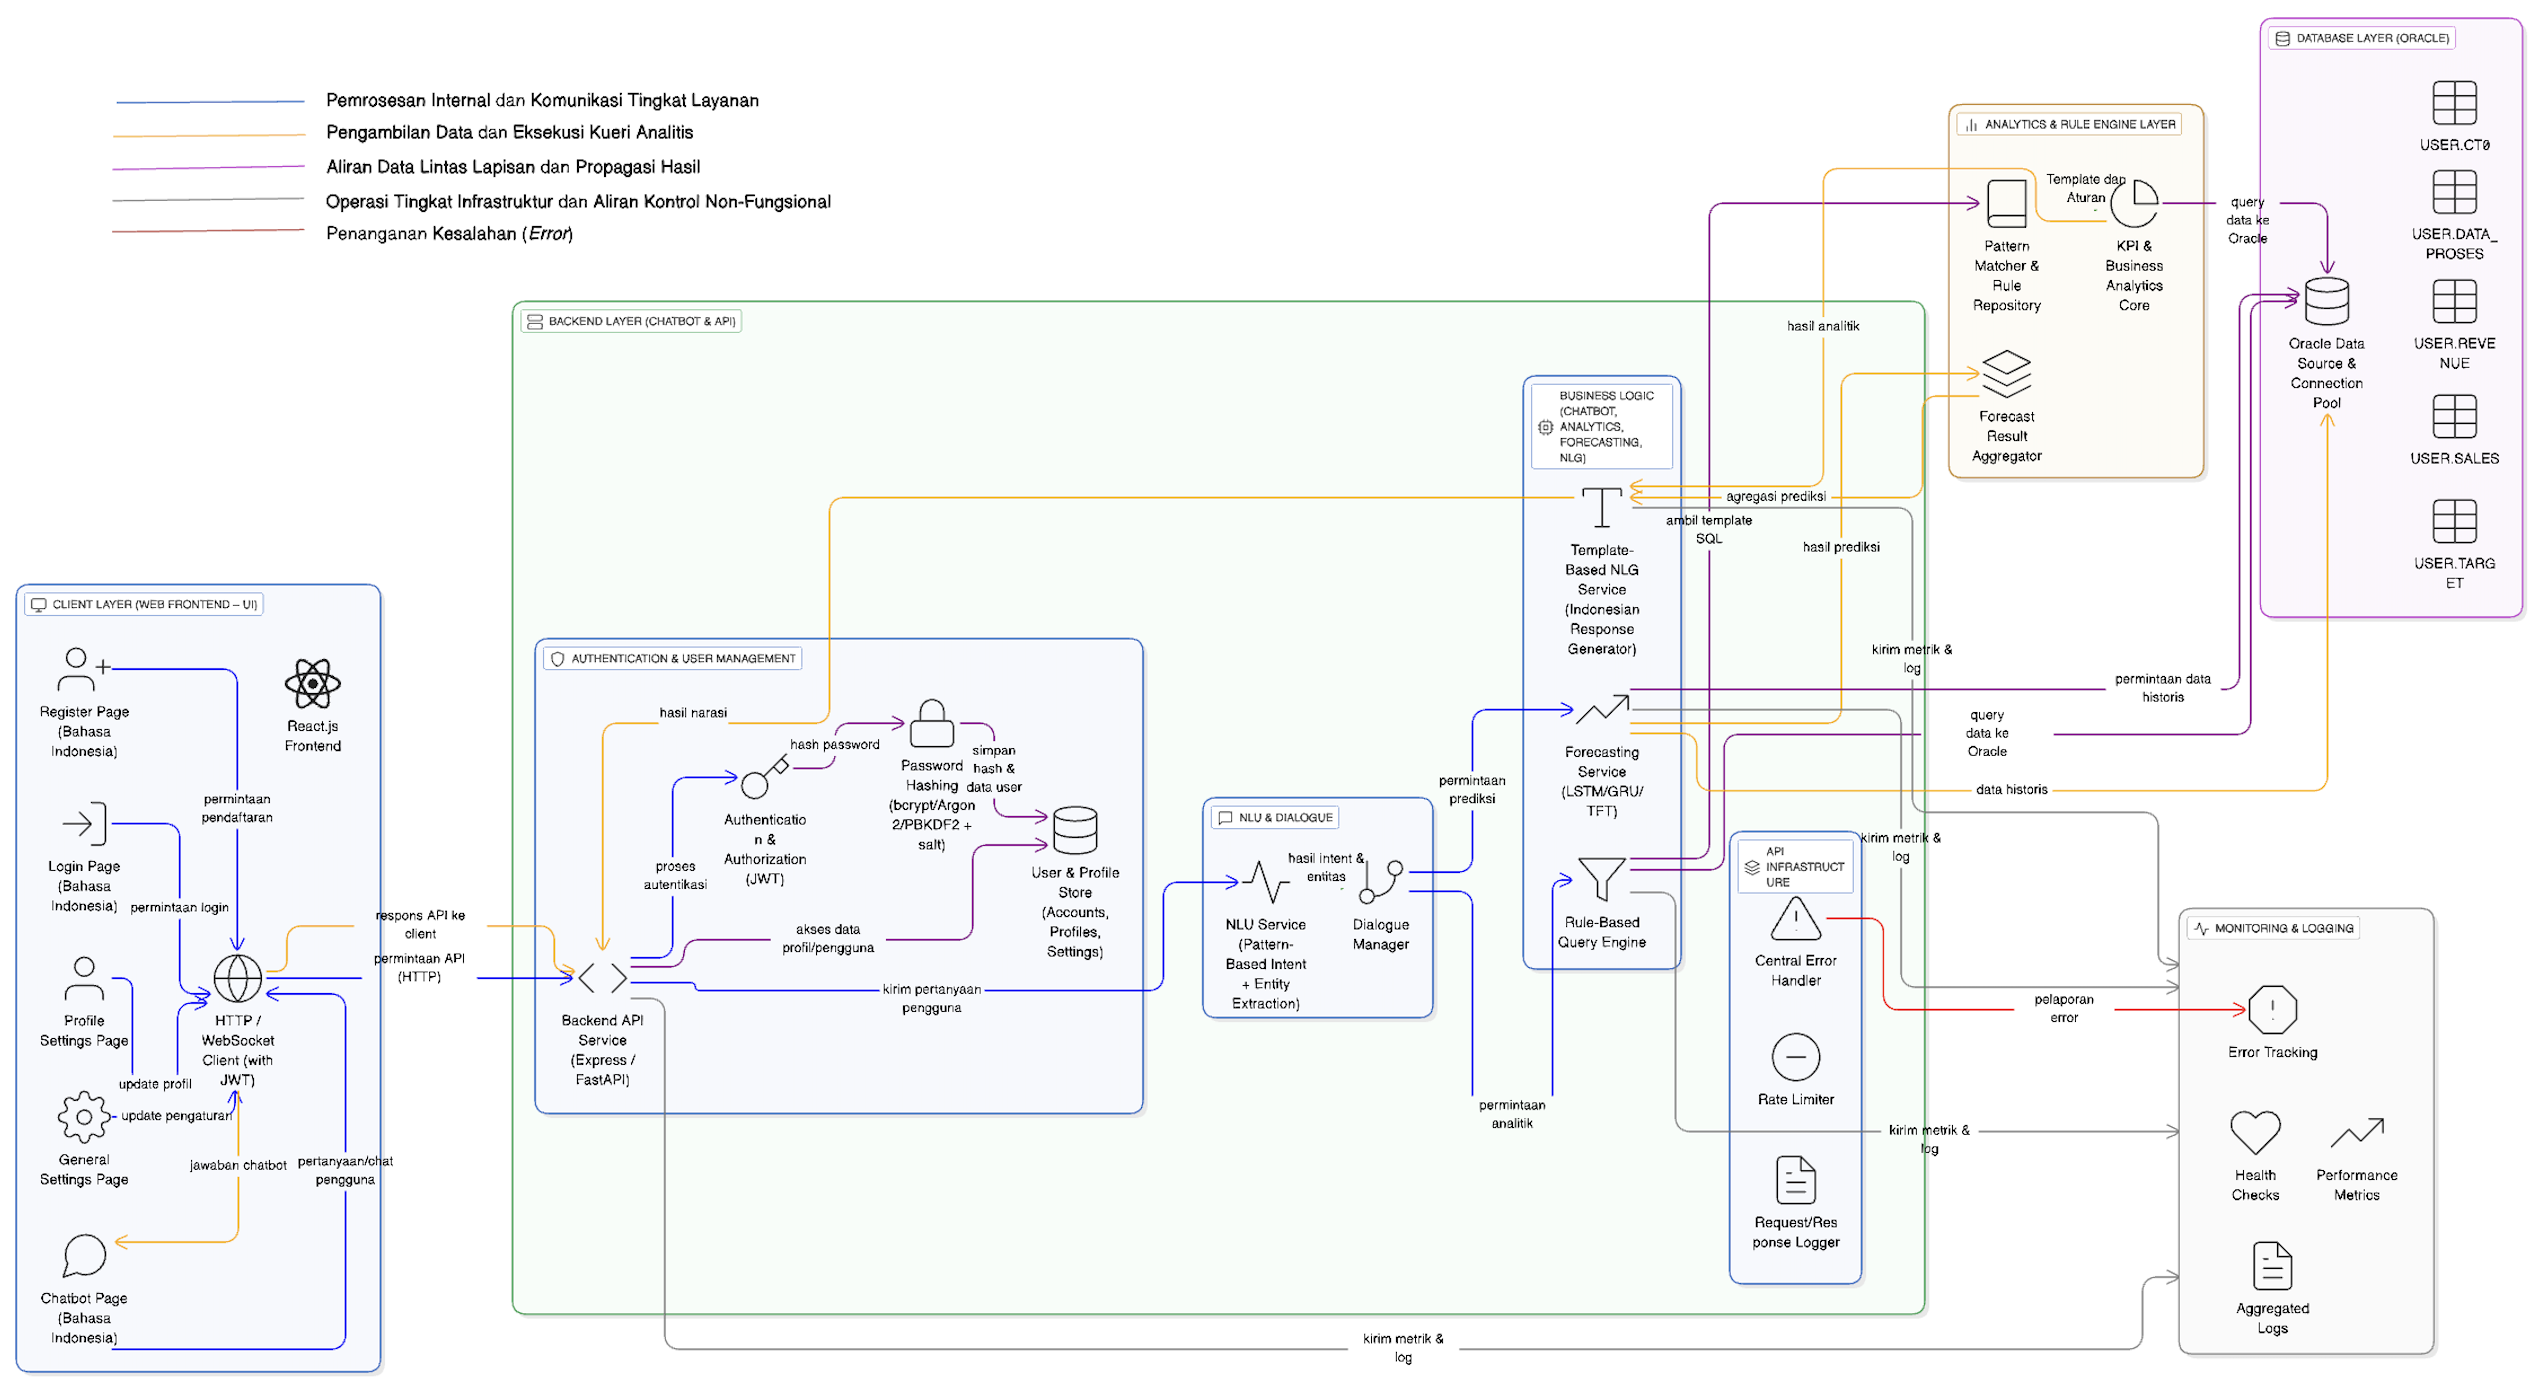
\includegraphics[width=1\textwidth,
                   height=1\textheight,
                   keepaspectratio]{images/arsitektur}
  \caption{Diagram Arsitektur Sistem Baru Secara Keseluruhan}
  \label{fig:arsitektur}
\end{figure}

Diagram arsitektur ini menggunakan sistem pewarnaan aliran untuk membedakan jenis interaksi yang terjadi antar komponen sehingga pembacaan terhadap alur kerja sistem menjadi lebih jelas. Aliran berwarna biru menggambarkan proses internal dan komunikasi tingkat layanan, yaitu interaksi antarmodul di dalam \textit{backend} seperti layanan autentikasi, modul klasifikasi maksud, manajemen dialog, mesin kueri berbasis aturan, serta layanan peramalan. Aliran berwarna oranye merepresentasikan proses pengambilan data dan eksekusi kueri analitik, khususnya komunikasi antara \textit{backend} dan \textit{Enterprise Data Warehouse} melalui sistem koneksi \textit{Oracle} untuk memperoleh data historis maupun metrik operasional yang relevan. Sementara itu, aliran berwarna ungu menunjukkan aliran data lintas lapisan dan propagasi hasil, yaitu bagaimana keluaran analitik dikembalikan ke lapisan logika bisnis untuk diproses lebih lanjut melalui mekanisme templating NLG. Aliran berwarna abu-abu menggambarkan operasi infrastruktur (seperti \textit{logging}, \textit{rate limiting}, pemantauan) yang dikelola oleh unit infrastruktur API guna menjaga keandalan sistem secara menyeluruh. Aliran berwarna merah digunakan untuk menandakan jalur penanganan kesalahan (\textit{error handling}). Melalui pemisahan aliran ini, diagram memberikan representasi yang lebih presisi mengenai bagaimana permintaan dari antarmuka diproses secara \textit{end-to-end}, mulai dari autentikasi, analisis \textit{intent}, eksekusi aturan, perhitungan prediktif, pengambilan data ke EDW, hingga penyusunan dan pengiriman kembali respons kepada pengguna.

Sebagai catatan komprehensif terhadap diagram arsitektur sistem di atas, komponen \textit{Temporal Fusion Transformer} (TFT) dicantumkan pada desain layanan peramalan sebagai bentuk rancangan sistem prediktif yang holistik. Akan tetapi, implementasi secara teknis pada penelitian ini difokuskan secara eksklusif pada pemodelan LSTM dan GRU. Model TFT diposisikan sebagai landasan teoretis untuk pengembangan iterasi sistem di masa mendatang mengingat tingginya kompleksitas komputasi serta besarnya kebutuhan volume data latih yang dipersyaratkan oleh arsitektur tersebut.

Dalam mencegah terjadinya latensi yang tinggi, aspek waktu respons ditetapkan sebagai salah satu metrik krusial dalam perancangan ini mengingat produk yang dikembangkan beroperasi pada level operasional dan harus mampu memberikan jawaban secara cepat terhadap permintaan analitik harian. Tantangan utama muncul dari karakteristik \textit{Enterprise Data Warehouse} yang menyimpan data dalam volume besar sehingga eksekusi kueri kompleks berpotensi menimbulkan penundaan. Dalam mengatasi hal tersebut, sistem menerapkan mekanisme optimasi, termasuk tembolok tingkat aturan (\textit{rule-level caching}) dengan pendekatan \textit{Time To Live} (TTL) yang memastikan hasil kueri disimpan sementara dan digunakan kembali tanpa perlu mengakses EDW setiap kali pengguna mengajukan permintaan yang sama. Kombinasi dari strategi ini memungkinkan penurunan latensi secara konsisten dan memastikan bahwa sistem tetap responsif dalam konteks penggunaan operasional.

\section{Kebutuhan Perangkat dan Lingkungan Sistem}
\label{sec:perangkat}

Dalam memastikan bahwa arsitektur yang dirancang dapat diimplementasikan dan direproduksi, sistem memerlukan spesifikasi perangkat lunak dan perangkat keras tertentu yang berfungsi sebagai fondasi dari pengembangan sistem (\textit{environment setup}).

\subsection{Perangkat Lunak dan Teknologi}
\label{subsec:tools}

Dalam melakukan implementasi dan pembangunan sistem yang nyata (tidak hanya sekadar rancangan), dibutuhkan beberapa perangkat lunak, pustaka pemrograman (\textit{libraries}), dan teknologi pendukung. Daftar teknologi pada Tabel~\ref{tab:tools} merincikan versi dan fungsi spesifik setiap perangkat dalam sistem \textit{Business Intelligence Chatbot}. Penjabaran ini memastikan bahwa seluruh proses, dari akuisisi data, pelatihan model, hingga rekayasa fitur, dapat ditelusuri dan direproduksi secara akurat.

\begin{longtable}{|c|p{2.5cm}|p{9cm}|}
\caption{Perangkat Lunak dan Teknologi Implementasi Sistem} \label{tab:tools} \\
\hline
\textbf{No} & \textbf{Perangkat} & \textbf{Deskripsi} \\
\hline
\endfirsthead
\multicolumn{3}{c}%
{\tablename\ \thetable\ -- \textit{Lanjutan dari halaman sebelumnya}} \\
\hline
\textbf{No} & \textbf{Perangkat} & \textbf{Deskripsi} \\
\hline
\endhead
\hline \multicolumn{3}{r}{\textit{Bersambung ke halaman berikutnya}} \\
\endfoot
\hline
\endlastfoot

1 & Node.js & \textit{Runtime} JavaScript sisi pelayan yang digunakan sebagai \textit{backend} utama sistem. Node.js menjalankan Express.js untuk menyediakan \textit{RESTful API}, mengelola autentikasi pengguna, mengeksekusi mesin aturan (\textit{rule engine}), serta menghasilkan respons naratif melalui modul NLG berbasis templat JavaScript. \\
\hline

2 & Python & Bahasa pemrograman yang digunakan khusus untuk layanan \textit{machine learning} (\textit{ML Service}). Python menangani pelatihan dan inferensi model peramalan deret waktu berbasis GRU dan LSTM melalui \textit{framework} FastAPI. \\
\hline

3 & FastAPI & \textit{Framework} Python untuk membangun \textit{RESTful API} dengan performa tinggi dan dokumentasi otomatis (Swagger/OpenAPI). FastAPI digunakan khusus untuk layanan \textit{machine learning} yang menangani permintaan pelatihan dan prediksi model peramalan deret waktu. \\
\hline

4 & React.js & Pustaka JavaScript untuk membangun antarmuka pengguna yang interaktif dan responsif. React.js digunakan untuk mengembangkan \textit{frontend chatbot} berbasis web dengan fitur percakapan, panel peramalan, dan alur terpandu (\textit{guided flow}). \\
\hline

5 & Oracle Database & \textit{Enterprise Data Warehouse} (DWH) yang menjadi sumber data utama sistem. Oracle Database digunakan untuk dua tujuan: (1) menyimpan data pengguna, riwayat percakapan, dan sesi melalui \textit{connection pooling} dengan pustaka \texttt{node-oracledb}; dan (2) menyediakan data analitik bisnis dari skema \texttt{DWH\_MOIS} yang mencakup lima domain data (penjualan, pendapatan, target, proses data pelanggan, dan \textit{churn}). \\
\hline

6 & PyTorch & \textit{Framework deep learning} utama yang digunakan untuk membangun dan melatih model peramalan deret waktu berbasis GRU dan LSTM. PyTorch dipilih karena fleksibilitas dalam pendefinisian arsitektur model kustom dan kemudahan \textit{debugging}. \\
\hline

7 & Express.js & \textit{Framework} web minimalis untuk Node.js yang digunakan sebagai fondasi \textit{backend} utama. Express.js menangani \textit{routing}, \textit{middleware} keamanan (Helmet, CORS, \textit{rate limiter}), serta integrasi dengan mesin aturan dan modul NLG. \\
\hline

8 & Pandas & Pustaka Python untuk manipulasi dan analisis data tabular. Pandas digunakan pada tahap \textit{data preparation}, transformasi fitur, dan agregasi data sebelum proses pelatihan model maupun eksekusi kueri. \\
\hline

9 & NumPy & Pustaka Python untuk komputasi numerik yang menjadi fondasi operasi matematika pada pemrosesan data dan perhitungan metrik evaluasi model. \\
\hline

10 & Scikit-learn & Pustaka \textit{machine learning} Python yang digunakan untuk praolah data, ekstraksi fitur, perhitungan metrik evaluasi, dan implementasi model \textit{baseline} untuk perbandingan performa. \\
\hline

11 & \texttt{node-oracledb} & Pustaka Node.js resmi dari Oracle untuk koneksi ke Oracle Database. Pustaka ini mengelola \textit{connection pooling}, eksekusi kueri SQL, dan penanganan tipe data khusus Oracle seperti CLOB. \\
\hline

12 & Regex (JavaScript) & Modul ekspresi reguler bawaan JavaScript yang digunakan untuk implementasi pencocokan pola (\textit{pattern matching}) dalam klasifikasi maksud berbasis aturan dan ekstraksi konteks geografis dari kueri pengguna. \\
\hline

13 & Pustaka Templat JavaScript & Modul templat kustom yang dibangun dalam JavaScript untuk implementasi \textit{template-based Natural Language Generation}. Modul ini mendukung lebih dari 30 subjek aturan dengan variasi templat per \textit{intent} yang diisi secara dinamis berdasarkan data hasil kueri Oracle. \\
\hline

14 & JWT / bcrypt & Pustaka keamanan yang digunakan untuk autentikasi berbasis \textit{JSON Web Token} (JWT) dan enkripsi kata sandi menggunakan algoritma \textit{bcrypt} dengan \textit{salt rounds}. \\
\hline

15 & Git / GitHub & Sistem kontrol versi dan platform kolaborasi yang digunakan untuk manajemen kode sumber, pelacakan perubahan, dan dokumentasi proyek tugas akhir. \\
\hline

16 & Jupyter Notebook & Aplikasi \textit{open-source} yang digunakan untuk eksplorasi data, eksperimen model, dan dokumentasi proses analisis dalam format dokumen interaktif yang menggabungkan kode, visualisasi, dan narasi. \\
\hline

17 & Google Colaboratory & Platform \textit{cloud} dari Google yang menyediakan akses gratis ke GPU untuk pelatihan model \textit{deep learning}. Google Colab digunakan untuk melatih model peramalan deret waktu yang memerlukan komputasi intensif. \\
\hline

18 & Postman & Aplikasi untuk pengujian dan dokumentasi API. Postman digunakan untuk menguji \textit{endpoint} API \textit{backend} sistem dan memvalidasi respons sebelum integrasi dengan \textit{frontend}. \\
\hline

19 & Visual Studio Code & \textit{Integrated Development Environment} (IDE) yang digunakan untuk penulisan kode, \textit{debugging}, dan manajemen proyek pengembangan sistem. \\
\hline

\end{longtable}


\subsection{Kebutuhan Sumber Daya Komputasi}
\label{subsec:resources}

Dalam mendukung proses pelatihan model \textit{deep learning} dan pengujian arsitektur yang diusulkan, diperlukan sumber daya komputasi yang memadai. Pelatihan model peramalan deret waktu berbasis LSTM dan GRU memerlukan akselerasi GPU untuk mempercepat proses komputasi yang kompleks. Pengembangan sistem ini memanfaatkan Google Colaboratory yang menyediakan akses ke GPU NVIDIA T4 dengan kapasitas 15GB memori GPU. 

Dalam tahap implementasi dan peluncuran produk secara langsung (\textit{deployment}), infrastruktur peladen (\textit{server}) dirancang untuk memiliki spesifikasi minimal 4 inti prosesor (\textit{cores}), memori RAM sebesar 16GB, dan penyimpanan berbasis SSD minimal 100GB guna memastikan aliran data yang cepat tanpa \textit{bottleneck} pada sistem berkas. 

\section{Desain Pengujian dan Evaluasi}
\label{sec:evaluasi}

Dalam memastikan bahwa sistem yang dikembangkan memenuhi spesifikasi dari desain arsitektur yang diajukan dan menguji keberhasilan implementasi, dirancang strategi pengujian dan evaluasi. Evaluasi ini mencakup penyelesaian bagian-bagian inti yang paling menantang dari sistem: modul klasifikasi maksud berbasis pola, pembangkitan bahasa alami (NLG), dan performa prediksi deret waktu.

\subsection{Evaluasi Klasifikasi Maksud Berbasis Pola}
\label{subsec:eval-intent}

Modul pencocokan kueri ke aturan bisnis dievaluasi menggunakan metrik standar klasifikasi multi-kelas. Sistem mengimplementasikan tujuh kategori \textit{intent} yang dipetakan ke 38 aturan bisnis; evaluasi dilakukan pada level pencocokan aturan (38 kelas) dengan pendekatan \textit{one-vs-all} dan agregasi metrik menggunakan strategi \textit{macro-averaging}, \textit{micro-averaging}, dan \textit{weighted-averaging}.

\subsubsection{Metrik Evaluasi Klasifikasi \textit{Intent}}

Metrik evaluasi yang digunakan untuk mengukur performa klasifikasi maksud mencakup:

\begin{enumerate}
    \item \textbf{Akurasi (\textit{Accuracy})}: Proporsi prediksi yang benar dari keseluruhan prediksi. Target minimal adalah 85\%.
    \item \textbf{Presisi (\textit{Precision})}: Proporsi prediksi positif yang benar dari seluruh prediksi positif. Dihitung per kelas kemudian diagregasi.
    \item \textbf{Daya Ingat (\textit{Recall})}: Proporsi sampel positif yang berhasil diprediksi benar dari seluruh sampel positif aktual.
    \item \textbf{Skor-F1 (\textit{F1-Score})}: Rata-rata harmonik dari presisi dan daya ingat, memberikan keseimbangan antara kedua metrik.
\end{enumerate}

Formula perhitungan metrik agregasi adalah sebagai berikut.

\begin{equation}
\label{sym:K}
\text{Presisi}_{\text{makro}} = \frac{1}{K} \sum_{i=1}^{K} \text{Presisi}_i
\end{equation}
\eqcaption{Presisi Makro}

\begin{equation}
\text{Daya Ingat}_{\text{makro}} = \frac{1}{K} \sum_{i=1}^{K} \text{Daya Ingat}_i
\end{equation}
\eqcaption{Daya Ingat Makro}

\begin{equation}
\text{Skor-F1}_{\text{makro}} = \frac{1}{K} \sum_{i=1}^{K} \text{Skor-F1}_i
\end{equation}
\eqcaption{Skor-F1 Makro}

dengan $K$ adalah jumlah kelas \textit{intent} dalam sistem.

\subsubsection{Analisis Nilai Keyakinan (\textit{Confidence Score})}

Sistem menggunakan mekanisme pemberian nilai keyakinan dalam rentang 0 hingga 100 untuk setiap prediksi klasifikasi maksud. Nilai dihitung melalui fungsi penjumlah bobot kata kunci primer dan pendukung yang cocok ($c = \min(100,\;\text{skor} \times 10)$). Ambang batas (\textit{threshold}) ditetapkan pada nilai 40 dengan ketentuan:
\begin{enumerate}
    \item Jika nilai keyakinan $\geq$ 40: Prediksi dianggap valid.
    \item Jika nilai keyakinan $<$ 40: Sistem meminta klarifikasi (\textit{fallback mechanism}).
\end{enumerate}

\subsection{Evaluasi Pembangkitan Bahasa Alami Berbasis Templat}
\label{subsec:eval-nlg}

Modul \textit{Natural Language Generation} (NLG) dievaluasi dari dua aspek: akurasi faktual dan evaluasi subjektif oleh pengguna internal.

\subsubsection{Akurasi Faktual}

Akurasi faktual dievaluasi dengan memverifikasi apakah seluruh nilai numerik dan informasi bisnis dalam respons NLG sesuai dengan hasil kueri dari basis data. Karena pendekatan NLG berbasis templat bersifat deterministik dan menyisipkan data langsung dari hasil kueri tanpa proses generatif, akurasi faktual dijamin secara arsitektural (Target: 100\%).

\subsubsection{Evaluasi Subjektif Berbasis Pengguna}

Kualitas keluaran NLG dinilai secara subjektif oleh pengguna internal perusahaan menggunakan kuesioner berskala Likert 1--5 pada empat dimensi utama:
\begin{enumerate}
    \item \textbf{Ketepatan Respons}: Menilai apakah jawaban yang diberikan sistem sesuai dengan data aktual.
    \item \textbf{Kejelasan Narasi}: Menilai apakah narasi, tabel, dan penjelasan yang dihasilkan sistem mudah dipahami.
    \item \textbf{Relevansi Analisis}: Menilai apakah \textit{insight} atau analisis yang diberikan sistem relevan dengan konteks pertanyaan pengguna.
    \item \textbf{Kemudahan Penggunaan}: Menilai apakah antarmuka dan alur interaksi sistem bersifat intuitif.
\end{enumerate}

\subsection{Evaluasi Peramalan Deret Waktu}
\label{subsec:eval-forecasting}

Model dievaluasi menggunakan protokol \textit{rolling-origin backtesting} untuk mencegah \textit{data leakage}. Evaluasi mencakup \textit{baseline} (ARIMA, Prophet) dan model utama (LSTM, GRU).

\begin{enumerate}
    \item \textbf{MAE (\textit{Mean Absolute Error})}: Rata-rata nilai absolut selisih prediksi dan aktual.
    \item \textbf{RMSE (\textit{Root Mean Squared Error})}: Akar kuadrat rata-rata kuadrat selisih.
    \item \textbf{sMAPE (\textit{Symmetric Mean Absolute Percentage Error})}:
    \begin{equation}
    \text{sMAPE} = \frac{100\%}{n} \sum_{i=1}^{n} \frac{|y_i - \hat{y}_i|}{(|y_i| + |\hat{y}_i|)/2}
    \end{equation}
    \eqcaption{sMAPE}

    \item \textbf{MASE (\textit{Mean Absolute Scaled Error})}:
    \begin{equation}
    \text{MASE} = \frac{\text{MAE}}{\frac{1}{n-1} \sum_{i=2}^{n} |y_i - y_{i-1}|}
    \end{equation}
    \eqcaption{MASE}
\end{enumerate}

Dalam mengukur peningkatan performa model terhadap garis dasar (\textit{seasonal naive}), dihitung \textit{skill score}:
\begin{equation}
\text{\textit{Skill Score}} = 1 - \frac{\text{MAE}_{\text{model}}}{\text{MAE}_{\text{baseline}}}
\end{equation}
\eqcaption{\textit{Skill Score}}
